\chapter{Assignment \#9}

\label{ch:ass9n}

\begin{fullwidth}

\begin{enumerate}
\item Write a user-defined MATLAB function that solves, with the shooting method in conjunction with the secant method, a second-order boundary value problem of the form:

\begin{equation*}
\frac{d^2y}{dx^2}+f(x)\frac{dy}{dx} + g(x)y = h(x)
\end{equation*}
for $a \le x \le b$ with $y(a)=Y_a$ and $y(b)=Y_b$, where $Y_a$ and $Y_b$ are constants.  For the function name and arguments use: \lstinline[style=myMatlab]{[x,y] = BVPShootSecant(Fx,Gx,Hx,a,b,n,Ya,Yb,Wa,Wb)}.  The input arguments \lstinline[style=myMatlab]{Fx}, \lstinline[style=myMatlab]{Gx}, and \lstinline[style=myMatlab]{Hx} are names for the functions that calculate $f(x)$, $g(x)$, and $h(x)$ respectively.  The arguments \lstinline[style=myMatlab]{a} and \lstinline[style=myMatlab]{b} define the domain if the solution, \lstinline[style=myMatlab]{n} is the number of subintervals, \lstinline[style=myMatlab]{Ya} and \lstinline[style=myMatlab]{Yb} are the boundary conditions, and \lstinline[style=myMatlab]{Wa} and \lstinline[style=myMatlab]{Wb} are the assumed slopes at $x=a$ that are used in the first two iterations of the Secant Methad.  Within the user-defined function \lstinline[style=myMatlab]{BVPShootSecant}, use the function \lstinline[style=myMatlab]{odesCRK4} that you created in Assignment \#8.  The secant method should be carried out until the absolute value of the true error at $x=b$ is smaller than 0.001.

\vspace{0.5cm}

\noindent Use this function to solve the following boundary value problem:
\begin{equation*}
\frac{d^2y}{dx^2}+2x\frac{dy}{dx}+5y-\cos{(3x)}=0, \ \ 0 \le x \le \pi
\end{equation*}
with boundary conditions: $y(0)=1.5$, and $y(\pi)=0$.  Use $n=100$, $W_a=-5$, and $W_b = -1.5$.  Create a well-formatted plot of the solution.


\pagebreak

\item A cylindrical pipe with inner radius 1 cm and the wall thickness 2.5 cm carries a fluid at a temperature of 600$^{\circ}$C. The outer wall of the pipe is at 25$^{\circ}$C.  The govering equation for the temperature distribution in the pipe wall is:
\begin{equation*}
r\frac{d^2T}{dr^2}+\frac{dT}{dr}=-500
\end{equation*}
subject to the boundary conditions $T(1)=600^{\circ}$C and $T(3.5)=25^{\circ}$C.  Solve for the temperature $T(r)$ and plot the temperature distribution.

\begin{figure}[h!]
\centering
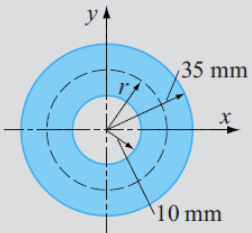
\includegraphics[width=5.0cm]{ass9n-p2.png}
\caption{Schematic of cylindrical pipe.}
\label{fig:ass9n-p2}
\end{figure}

\begin{enumerate}
\item
\begin{enumerate}
\item Solve using\lstinline[style=myMatlab]{BVPShootSecant} that you created for the first problem.
\item Solve using \lstinline[style=myMatlab]{bvp5c}.
\end{enumerate}
Plot the solution using both methods and output the value for $\frac{dT}{dr}\Bigl|_{r=3.5}$ using both methods.

\item 
What is the physical significance of the right-hand side (-500) in the governing equation?  (i.e. what conservation law is being expressed with the governing equation?) What happens to the temperature profile when the right-hand side is made much bigger?

\item 
Replace the boundary condition at $r=3.5$cm to model convective heat transfer to a fluid medium maintained at 25$^{\circ}$C.  Assume a convective heat transfer coefficient of 1.5 W/cm$^2$-K.  
\begin{equation*}
\frac{dT}{dr}\Bigl|_{r=3.5}=-h\left[T(3.5)-25\right]
\end{equation*}
Solve the problem using \lstinline[style=myMatlab]{bvp5c}, plot the temperature profile and output $T(r=3.5)$.  Experiment with different values of the convective heat transfer coefficient to make sure the response is as you expect.  What happens as the convective heat transfer coefficient gets very large?  What happens when it gets small?  Briefly describe your observation.


\end{enumerate}

\pagebreak

\item The radial distribution of temperature in a current-carrying bare wire is described by:
\begin{equation*}
\frac{k}{r}\frac{d}{dr}\left(r \frac{dT}{dr}\right)=-\frac{I^2 \rho_e}{\left(\frac{1}{4}\pi D^2 \right)^2}
\end{equation*}
where $T$ is the temperature in K, $r$ is the radial coordinate in meters, $k=72$ W/m/K is the thermal conductivity, $I=0.5$A is the current, $\rho_e=32\times 10^{-8}, \ \Omega-$m is the electrical resistivity, and $D=1 \times 10^{-4}$m is the wire diameter. Use MATLAB's built-in function \lstinline[style=myMatlab]{bvp5c} to solve the equation for $T(r)$.  Solve twice for the following boundary conditions.
\begin{enumerate}
\item at $r=10^{-6}$m, $\frac{dT}{dr}=0$ and $r= D/2, \ T=300$K.
\item at $r=10^{-6}$m, $\frac{dT}{dr}=0$ and at $r=D/2$, $\frac{dT}{dr}=-\frac{h}{k}\left(T(D/2)-T_{\infty}\right)$, where $h=100$ W/m$^{2}$-K is the convective heat transfer coefficient and $T_{\infty}=300$K is the ambient temperature.
\end{enumerate}

\vspace{0.25cm}

\noindent \textbf{Important note:} $r=0$ is a singular point and therefore must be replaced with a small, non-zero value, for example $10^{-6}$.  As initial guesses, use $T=500$K and $\frac{dT}{dr}=0$, use 50 subintervals.

\vspace{0.25cm}

\noindent For both parts a) and b), plot the temperature profiles and output the difference in temperature between the centerline of the wire and the outer surface of the wire.  Give a brief physical explanation for the differences in the temperature profiles for part a) and b).  

\end{enumerate}



\end{fullwidth}
